
\chapter{Reading the HDF5 Level-1 Files}

We assume that the reader is familiar with installing Python packages using either ``pip
install`` or Anaconda. This software has been tested using a default Anaconda stack with Python
version 3.7. In this chapter we will give a very brief overview of how to read the HDF5
files. Subsequent chapters will provide details on specific topics.

This code snippet illustrates how to read the level-1 data from spectral window 7 (containing
\ion{Fe}{12} 195.12\,\AA) in Python. Later in this chapter we'll show how to map a wavelength to a
window number.

\begin{lstlisting}
import h5py
import numpy as np

file_data = 'eis_20190404_131513.data.h5'
file_head = 'eis_20190404_131513.head.h5'

f_data = h5py.File(file_data, 'r')
data = np.array(f_data['level1/win07'])
f_data.close()
\end{lstlisting}
The resulting array is \verb+(512, 87, 24)+. That is, 512 pixels along the slit, 87 steps in the x
direction, and 24 pixels in the dispersion direction.

Information from the header file is read in a similar way. For example,
\begin{lstlisting}
f_head = h5py.File(file_head, 'r')
x_scale, = f_head['pointing/x_scale']
date_obs, = f_head['index/date_obs']
wave = np.array(f_head['wavelength/win07'])
radcal = np.array(f_head['radcal/win07_pre'])
f_head.close()
date_obs = date_obs.decode('utf-8')
\end{lstlisting}
Here \verb+x_scale+ is the number of arcsec per step in the raster. Most EIS rasters take more than
1 arcsec per step, which degrades the spatial resolution but increases the cadence. The variable
\verb+radcal+ is the pre-flight calibration curve for this data window. It includes all of the
factors for converting counts directly to erg cm$^{-2}$ s$^{-1}$ sr$^{-1}$. The \verb+decode+ on
\verb+date_obs+ converts from a byte array to unicode.

We can make a quick image by summing the data in the dispersion direction. The
raster is scaled logarithmically.
\begin{lstlisting}
import matplotlib.pyplot as plt

raster = np.sum(data, axis=2)
range = np.percentile(raster, (1, 99))
range = range[1]*np.array([1.0E-2, 1.0])
scaled = np.clip(raster, range[0], range[1])
scaled = np.log10(raster)

plt.imshow(scaled, origin='lower', aspect=1/x_scale, cmap='gray')
plt.title(date_obs)
plt.show()
\end{lstlisting}
\begin{marginfigure}
  \centerline{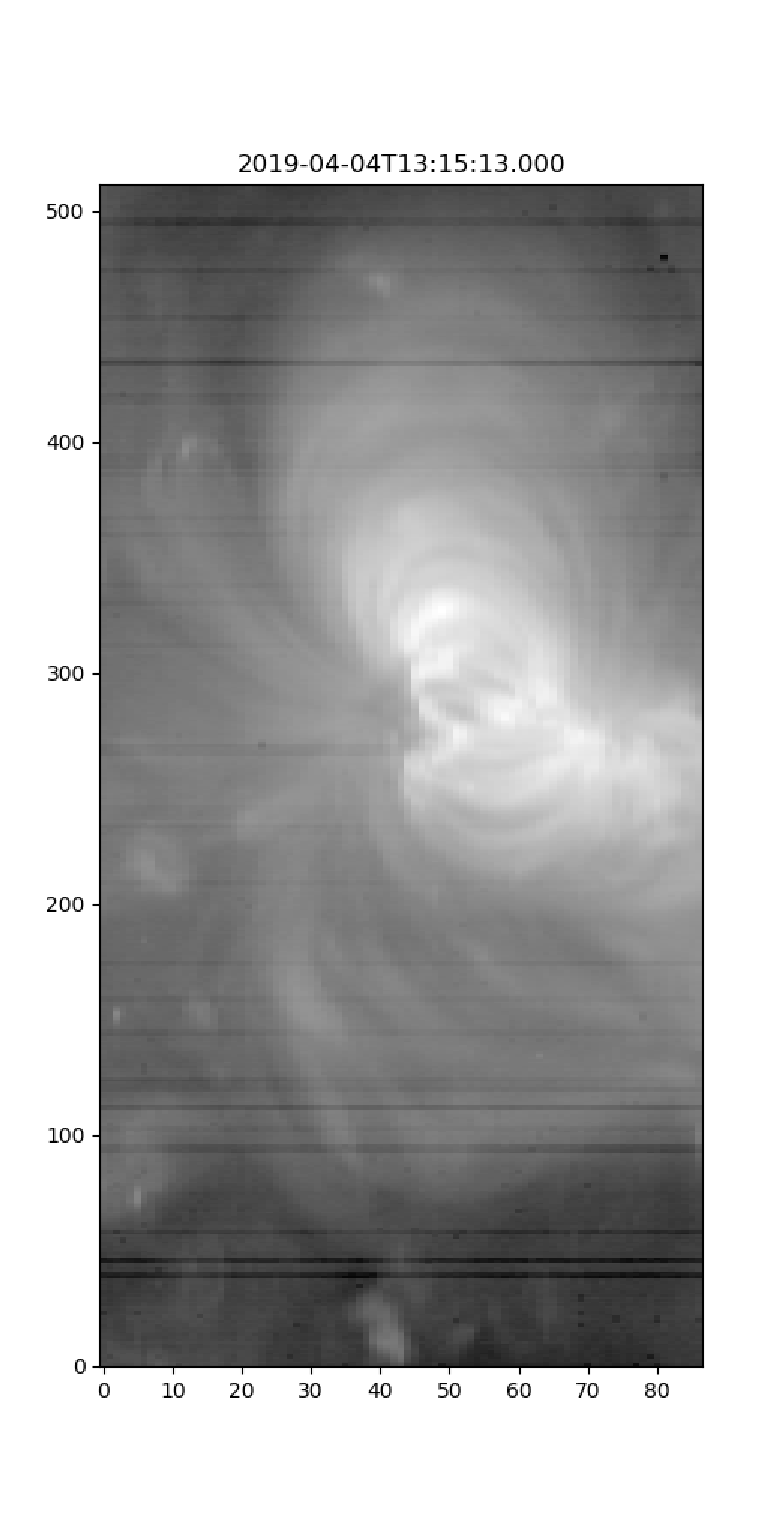
\includegraphics[clip,width=\linewidth]{figures/test_imshow.pdf}}
  \caption{An example image formed by summing the data for the \ion{Fe}{12} spectral window in the
    dispersion direction. In a subsequent chapter we'll discuss fitting the spectra.}
  \label{fig:raster}
\end{marginfigure}

The following code illustrates how to display the spectrum from a single pixel. To convert from
counts to calibrated units we simply multiply by the calibration curve. Note how the array is
addressed differently in Python than in IDL.
\begin{lstlisting}
ix = 48
iy = 326
spec = data[iy, ix, :]
spec_cal = spec*radcal

plt.subplot(1, 2, 1)
plt.plot(wave, spec)
plt.title('units = counts')

plt.subplot(1, 2, 2)
plt.plot(wave, spec_cal)
plt.title('units = ergs cm$^{-2}$ s$^{-1}$ sr$^{-1}$')

plt.show()
\end{lstlisting}
\begin{marginfigure}
  \centerline{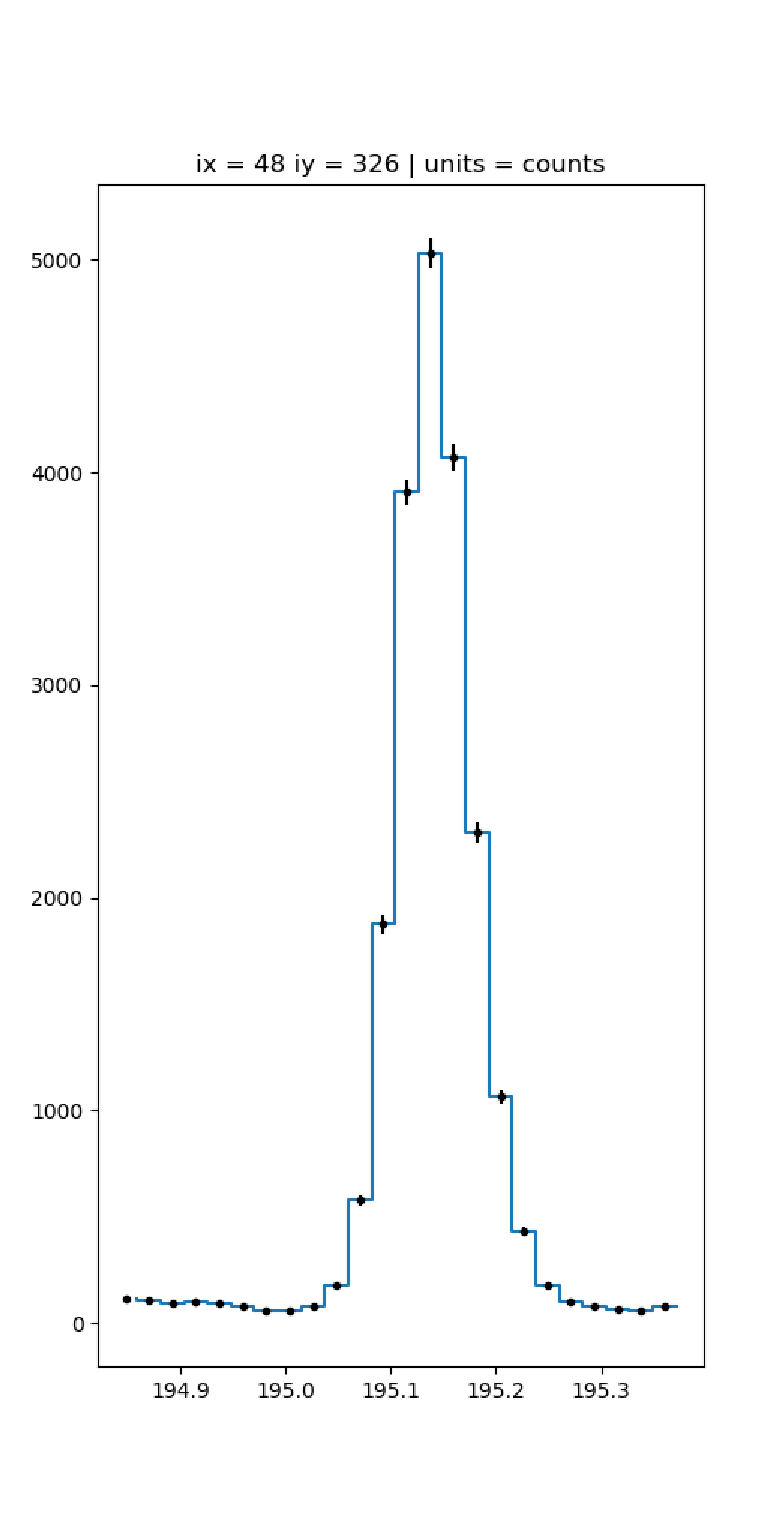
\includegraphics[clip,width=\linewidth]{figures/test_plot.pdf}}
  \caption{An example \ion{Fe}{12} 195.119\,\AA\ line profile from the raster.}
  \label{fig:spectrum}
\end{marginfigure}

We usually don't care about the numbering of the data windows. It's more natural to want to read
the data corresponding to a particularly wavelength. The data in the \verb+wininfo+ group contains
the max and min wavelengths for each data window and allows us to map from wavelength to window
number.
\begin{lstlisting}
f_head = h5py.File(file_head, 'r')
nwin, = f_head['/wininfo/nwin']
dt = np.dtype([('line_id', 'U64'), ('wvl_min', 'f'), ('wvl_max','f')])
wininfo = np.zeros((nwin,), dtype=dt)
wininfo = wininfo.view(np.recarray)
for iwin in range(nwin):
    line_id, = f_head[f'/wininfo/win{iwin:02d}/line_id']
    wvl_min, = f_head[f'/wininfo/win{iwin:02d}/wvl_min']
    wvl_max, = f_head[f'/wininfo/win{iwin:02d}/wvl_max']
    wininfo[iwin].line_id = line_id.decode('utf-8')
    wininfo[iwin].wvl_min = wvl_min
    wininfo[iwin].wvl_max = wvl_max
f_head.close()
\end{lstlisting}
Given a wavelength we can find the window number using the wavelength ranges for each window. Note
that we've converted \verb+wininfo+ to a numpy record array, which behaves similarly to an array of
IDL structures.
\begin{lstlisting}
wvl = 195.119
p = (wininfo.wvl_max - wvl)*(wvl - wininfo.wvl_min)
iwin, = np.where(p >= 0)
\end{lstlisting}
If the result is an empty list, the wavelength is not in the data.

Two final notes on reading the data. First, the contents of the HDF5 files can be displayed using
\verb+h5dump+, which is provided with Anaconda. For example,

\begin{lstlisting}
> h5dump -n eis_20190404_131513.data.h5
FILE_CONTENTS {
group      /
group      /level1
dataset    /level1/intensity_units
dataset    /level1/win00
dataset    /level1/win01
dataset    /level1/win02
dataset    /level1/win03
dataset    /level1/win04
dataset    /level1/win05
. . .
\end{lstlisting}
The actual data associated with each variable can be printed out using the \verb+-d+ option. For
example,
\begin{lstlisting}
> h5dump -d exposure_times/duration eis_20190404_131513.head.h5
HDF5 "eis_20190404_131513.head.h5" {
DATASET "exposure_times/duration" {
   DATATYPE  H5T_IEEE_F32LE
   DATASPACE  SIMPLE { ( 87 ) / ( 87 ) }
   DATA {
   (0): 40.0005, 40.0002, 40.0004, 40.0004, 39.9994, 40.0002, 39.9995, 40,
   (8): 40.0007, 39.9999, 40.0005, 40.0004, 39.9997, 40.0002, 39.9994,
   . . .
}
\end{lstlisting}
Second, there is a Python object \verb+eis_read_raster.py+ that can be used to read the data and head
files. For example,
\begin{lstlisting}
from eis_read_raster import eis_read_raster
filename = 'eis_20190404_131513.data.h5'
wave = 195.119
eis = eis_read_raster(filename, wave)
print(eis.data['index']['date_obs'])
print(eis.data['data'].shape)
\end{lstlisting}
In the chapters that follow we will use the object to do most of the heavy lifting. The routine
\verb+eis_display_window.py+ illustrates how to use the object and matplotlib to click around the
raster and display individual line profiles

\begin{figure}[t]
  \centerline{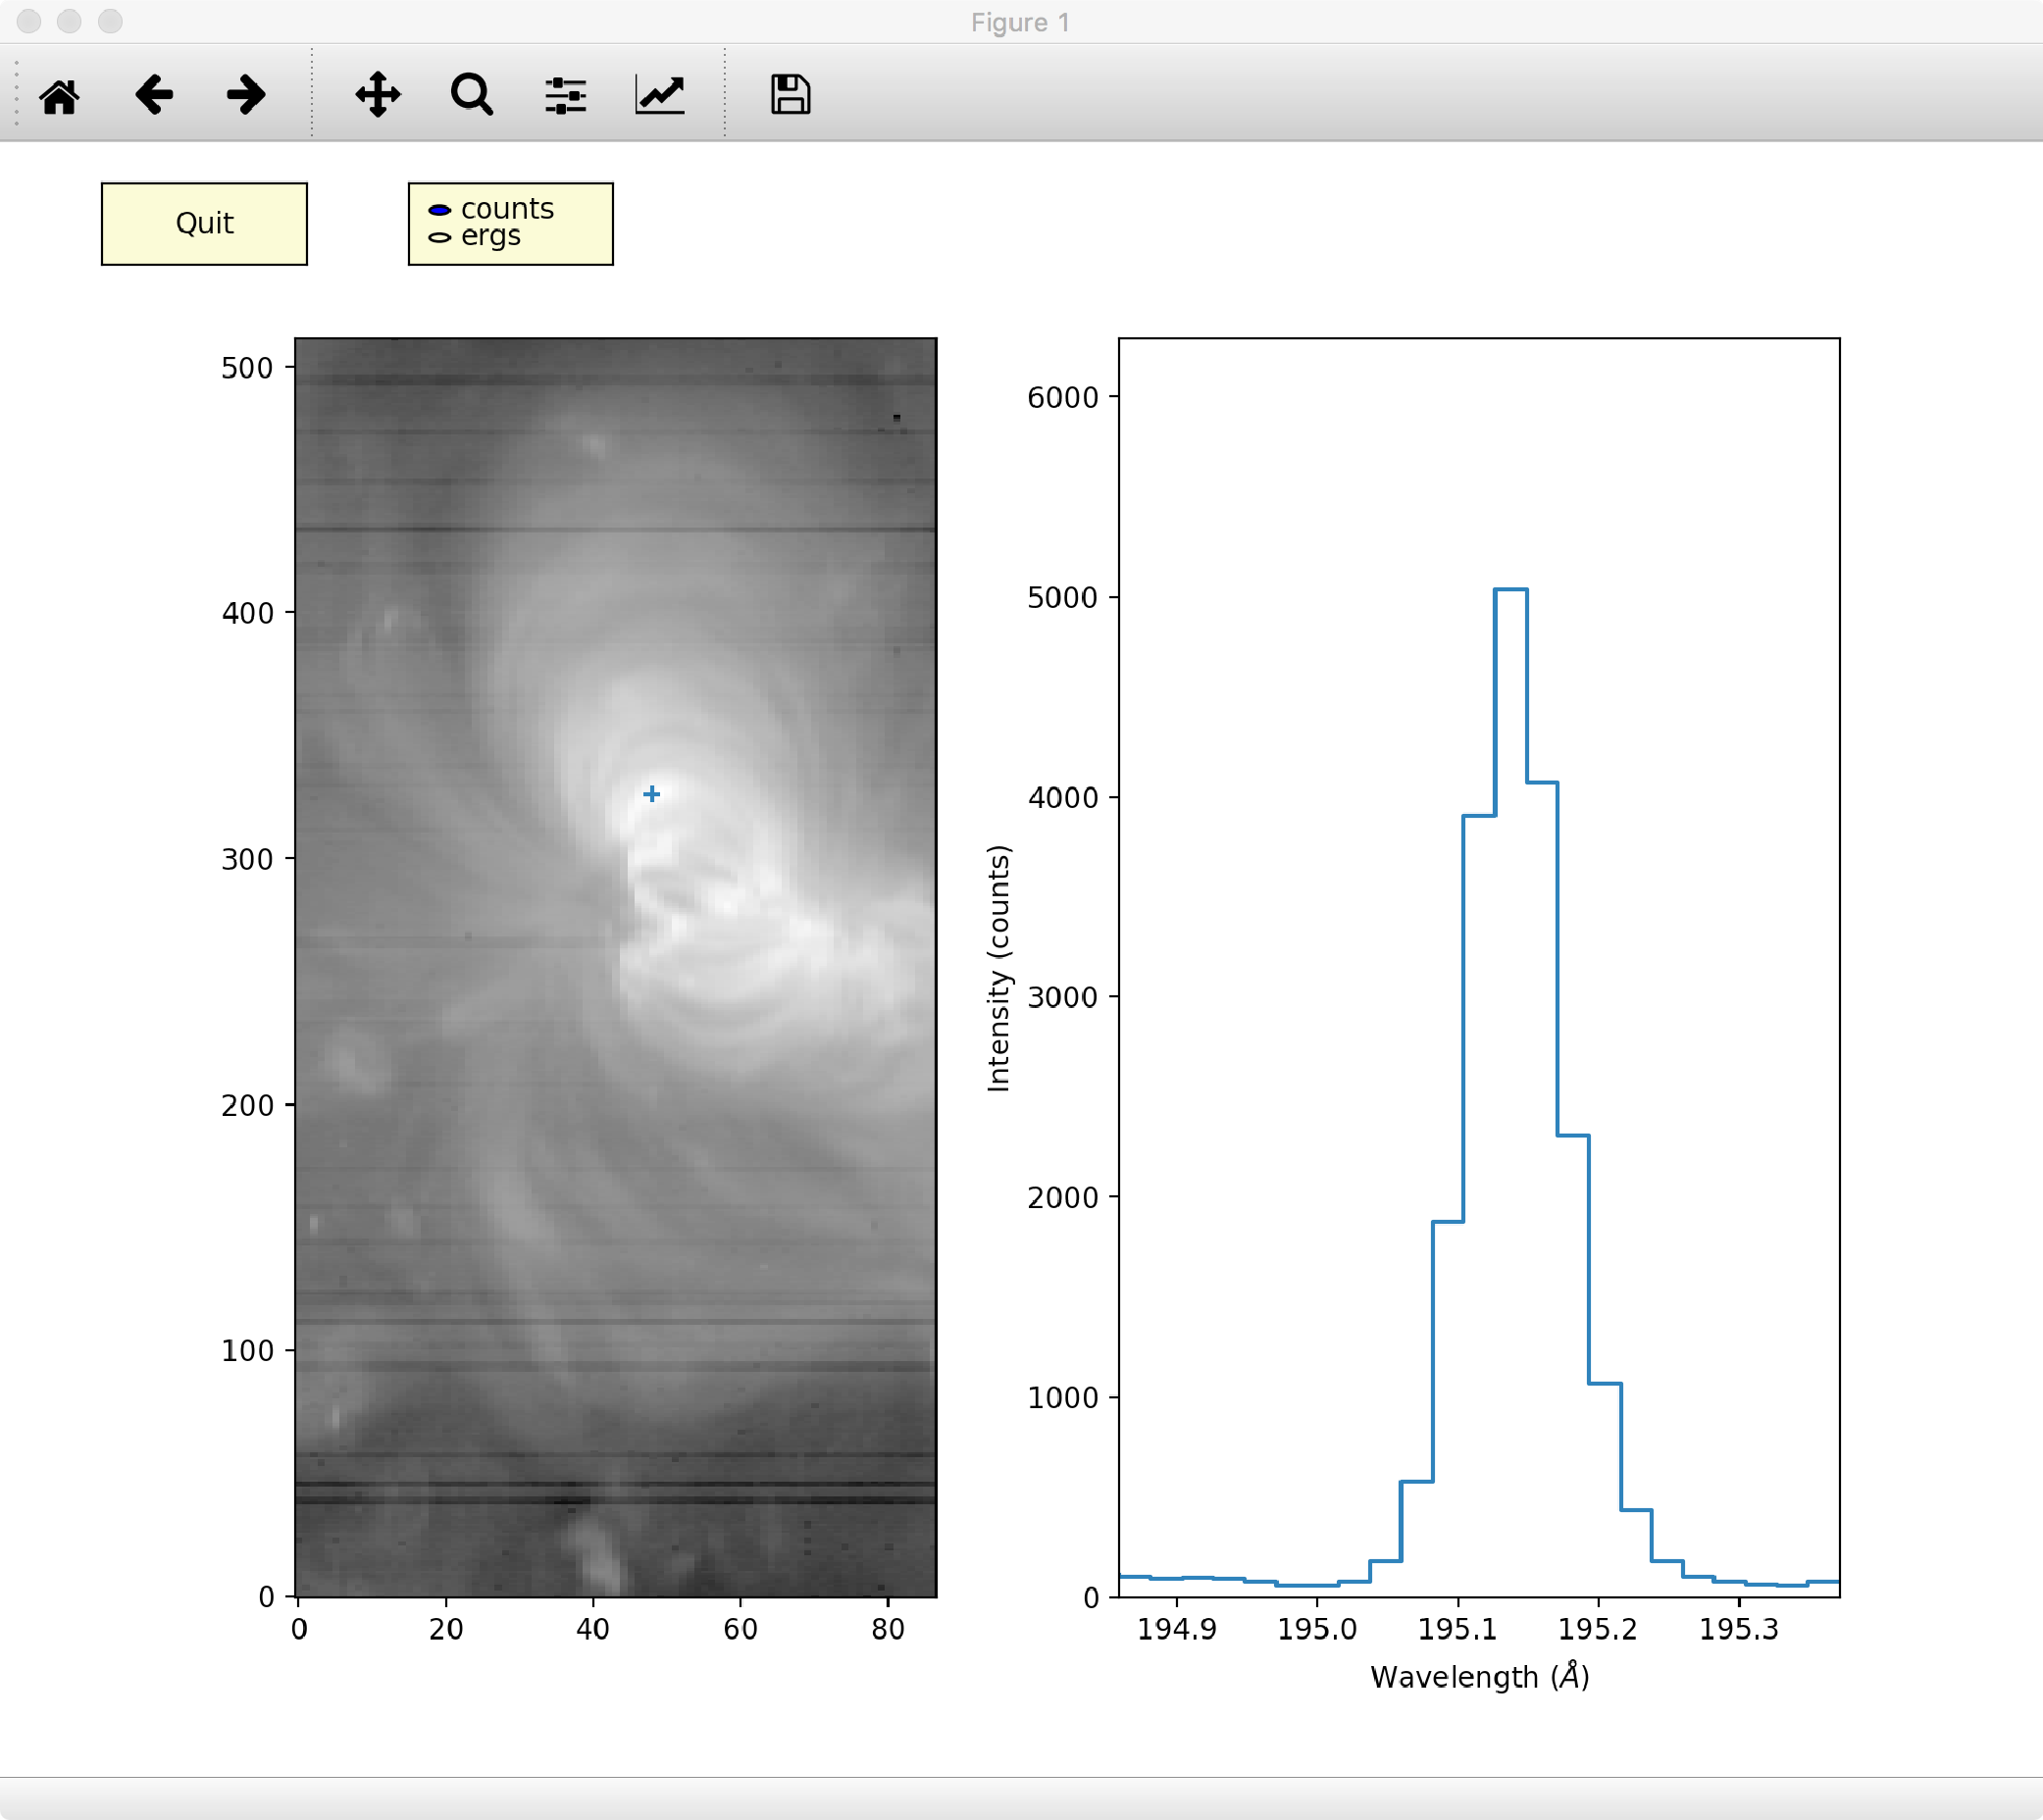
\includegraphics[clip,width=\linewidth]{figures/eis_display_window.pdf}}
  \caption{An example interactive plot showing the raster and the line profile at the selected
    position.}
  \label{fig:matplotlib}
\end{figure}
